\documentclass[11pt]{beamer}
\usetheme{Boadilla}
\usepackage[utf8]{inputenc}
\usepackage{amsmath}
\usepackage{amsfonts}
\usepackage{tikz}
\usetikzlibrary{snakes}
\usepackage{amssymb}
\date{2021-01-20}
\author{Simon-Pierre Boucher}
\title{Mathématiques Financières des Obligations}
\institute{Université Laval}


\begin{document}

\begin{frame}
\titlepage
\end{frame}

%\begin{frame}
%\tableofcontents
%\end{frame}

\begin{frame}{Équivalence de taux}
\begin{block}{Taux d'Intérêt Effectif}
\begin{itemize}
\item Notation : $r$
\item Il s'agit du taux utilisé dans le calcul de la capitalisation et de l'actualisation. 
\item Il s'agit également du taux réellement reçu sur un investissement $P_0$ et rapportant $I$ en intérêt.
\end{itemize}
\begin{align*}
I=P_0 \times r
\end{align*}
\end{block}
\end{frame}


\begin{frame}{Équivalence de taux}
\begin{block}{Taux d'Intérêt Nominal}
\begin{itemize}
\item Notation : $(i;m)$
\item Sera toujours accompagné d'un valeur $m$ représentant le nombre de capitalisation par période.
\item Il ne doit pas être utilisé dans les calculs d’actualisation et de capitalisation
\end{itemize}
\end{block}
\end{frame}


\begin{frame}{Équivalence de taux}
\begin{block}{Relation entre Taux d'Intérêt Nomina et taux d'intérêt effectif}
Le taux d'intérêt effectif $r$ est une fonction de notre taux d'intérêt nominal $i$ et de notre nombre de capitalisation par période. 
\begin{align*}
r=\frac{i}{m}
\end{align*}
\end{block}
\end{frame}

\begin{frame}{Taux effectif $\rightarrow$ Taux effectif}
Transformer un taux effectif $r_2$ en un autre taux effectif $r_1$ à l'aide de l'équation suivante:
\begin{align*}
r_1 =(1+r_2)^{\frac{u}{v}}-1
\end{align*}
Sachant 
\begin{itemize}
\item $r_1$ est le taux effectif par $u$ période 
\item $r_2$ est le taux effectif par $v$ période 
\end{itemize}
\end{frame}

\begin{frame}{Taux effectif $\rightarrow$ Taux effectif}
Voici les valeurs prises par $u$ et $v$ lorsque nous avons les taux effectifs suivants 


\begin{table}[H]
\begin{center}
\begin{tabular}{|c|c|l|l|}
\hline
\multicolumn{1}{|l|}{\textbf{$r_1$}} & \multicolumn{1}{l|}{\textbf{$r_2$}} & \textbf{$u$} & \textbf{$v$} \\ \hline
\textbf{Quotidien}                   & \textbf{Annuel}                     & 1            & 365          \\ \hline
\textbf{Hebdomadaire}                & \textbf{Annuel}                     & 1            & 52           \\ \hline
\textbf{Mensuel}                     & \textbf{Annuel}                     & 1            & 12           \\ \hline
\textbf{Trimestriel}                 & \textbf{Annuel}                     & 1            & 4            \\ \hline
\textbf{Semestriel}                  & \textbf{Annuel}                     & 1            & 2            \\ \hline
\textbf{Quotidien}                   & \textbf{Semestriel}                 & 2            & 365          \\ \hline
\textbf{Hebdomadaire}                & \textbf{Semestriel}                 & 2            & 52           \\ \hline
\textbf{Mensuel}                     & \textbf{Semestriel}                 & 2            & 12           \\ \hline
\textbf{Trimestriel}                 & \textbf{Semestriel}                 & 2            & 4            \\ \hline
\end{tabular}
\end{center}
\end{table}
\end{frame}

\begin{frame}{Taux effectif $\rightarrow$ Taux nominal}
Transformer un taux effectif $r$ en un taux nominal $(i;m)$ à l'aide de l'équation suivante:
\begin{align*}
i = r \times m
\end{align*}
\end{frame}

\begin{frame}{Taux nominal $\rightarrow$ Taux effectif}
Transformer un taux nominal $(i;m)$ en un taux effectif $r$ à l'aide de l'équation suivante:
\begin{align*}
r=\frac{i}{m}
\end{align*}
\end{frame}

\begin{frame}{Capitalisation et Actualisation}
\begin{block}{Valeur Future (Capitalisation)}
Dans cette section, nous allons regarder comment capitaliser un montant unique. La capitalisation nous permet de déterminer la valeur future d'un montant d'argent investit aujourd'hui à un taux spécifié. Voici les paramètres que nous utiliserons:
\begin{itemize}
\item $P_0=$ Montant investi en $t=0$ 
\item $r=$ Taux d'intérêt périodique reçu sur l'investissement
\item $n=$ Période pendant lequel le montant initial est investi
\item $P_n=$ Valeur future de notre investissement $P_0$ en $t=n$
\end{itemize}
Voici l'équation nous permettant de trouver la valeur future de notre investissement 
\begin{align*}
P_n=P_0 \times (1+r)^n
\end{align*}
\end{block}
\end{frame}

\begin{frame}{Capitalisation et Actualisation}
\begin{block}{Valeur Présente (Actualisation)}
Dans cette section, nous allons regarder comment actualiser un montant unique. L'actualisation nous permet de déterminer la valeur présente d'un montant d'argent que nous allons recevoir dans le future. Voici les paramètres que nous utiliserons:
\begin{itemize}
\item $P_0=$ Montant à recevoir dans le futur en valeur d'aujourd'hui ($t=0$), soit la valeur présente  
\item $r=$ Taux d'intérêt périodique en vigueur dans l'économie
\item $n=$ Nombre de périodes avant que le montant soit reçu.
\item $P_n=$ Montant nominal à recevoir dans le futur ($t=n$)
\end{itemize}
Voici l'équation nous permettant de trouver la valeur présente d'un montant à recevoir dans le futur.
\begin{align*}
P_0=\frac{P_n}{(1+r)^n}
\end{align*}
\end{block}
\end{frame}

\begin{frame}{Annuité}

Une annuité est tout simplement une suite de paiements identiques et reçus à intervalle constant pendant une période spécifiée. Voici une ligne du temps représentant une annuité.
\vspace{1cm}

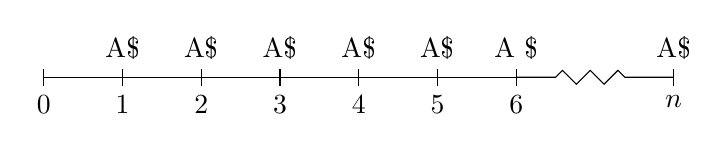
\begin{tikzpicture}[snake=zigzag, line before snake = 5mm, line after snake = 5mm]
    % draw horizontal line   
    \draw (0,0) -- (6,0);
    \draw[snake] (6,0) -- (8,0);

    % draw vertical lines
    \foreach \x in {0,1,2,3,4,5,6,8}
      \draw (\x cm,3pt) -- (\x cm,-3pt);

    % draw nodes
    \draw (0,0) node[below=3pt] {$ 0 $} node[above=3pt] {$   $};
    \draw (1,0) node[below=3pt] {$ 1 $} node[above=3pt] {A\$};
    \draw (2,0) node[below=3pt] {$ 2 $} node[above=3pt] {A\$};
    \draw (3,0) node[below=3pt] {$ 3 $} node[above=3pt] {A\$};
    \draw (4,0) node[below=3pt] {$ 4 $} node[above=3pt] {A\$};
    \draw (5,0) node[below=3pt] {$ 5 $} node[above=3pt] {A\$};
    \draw (6,0) node[below=3pt] {$ 6 $} node[above=3pt] {A \$};
    \draw (7,0) node[below=3pt] {$  $} node[above=3pt] {$  $};
    \draw (8,0) node[below=3pt] {$ n $} node[above=3pt] {A\$};
  \end{tikzpicture}
  \vspace{0.5cm}
\begin{itemize}
\item $A\$$ représente le paiement reçu à chaque période 
\item $n$ représente le nombre de paiements que versera l'annuité
\end{itemize}
\end{frame}


\begin{frame}{Valeur future d'une annuité régulière}
La valeur future d'une annuité régulière, nous donnera la valeur de la somme de tous les flux $A\$$ capitalisé à $t=n$. $VF_{P_n}$ sera la notation que nous utiliserons pour la valeur future d'une annuité régulière. L'équation suivante montre comment obtenir la valeur future de notre annuité régulière.  
\begin{align*}
VF_{P_n} = A \times (1+r)^{n-1}+A \times (1+r)^{n-2}+....\\+A \times (1+r)^{1}+A \times (1+r)^{0}
\end{align*}
\end{frame}


\begin{frame}{Valeur future d'une annuité régulière}
Si le nombre de période $n$ est relativement faible, il sera simple de calculer la valeur future. Cependant, si nous avons un nombre important de périodes $n$, la formule suivante est plus pratique. 
\begin{align*}
VF_{P_n}=A \left[\frac{(1+r)^n-1}{r} \right]
\end{align*}
Sachant les paramètres suivants: 
\begin{itemize}
\item $VF_{P_n}=$ Valeur future d'une annuité régulière 
\item $A=$ flux monétaire constant reçu à chaque période  
\item $n=$ Nombre de flux monétaire qui sera versé dans cette annuité régulière
\item $r=$ taux d'intétêt périodique en vigueur 
\end{itemize}
\end{frame}



\begin{frame}{Valeur présente d'une annuité régulière}
La valeur présente d'une annuité régulière, nous donnera la valeur de la somme de tous les flux $A\$$ actualisé en $t=0$. $VP_{P_0}$ sera la notation que nous utiliserons pour la valeur présente d'une annuité régulière. L'équation suivante montre comment obtenir la valeur présente de notre annuité régulière.  
\begin{align*}
VP_{P_0} = \frac{A}{(1+r)^{1}}+\frac{A}{(1+r)^{2}}+....+\frac{A}{(1+r)^{n-1}}+\frac{A}{(1+r)^{n}}
\end{align*}
\end{frame}


\begin{frame}{Valeur présente d'une annuité régulière}
Si le nombre de période $n$ est relativement faible, il sera simple de calculer la valeur présente. Cependant, si nous avons un nombre important de périodes $n$, la formule suivante est plus pratique. 
\begin{align*}
VP_{P_0}=A \left[ \frac{1-\frac{1}{(1+r)^n}}{r} \right]
\end{align*}
Sachant les paramètres suivants: 
\begin{itemize}
\item $VP_{P_0}=$ Valeur présente d'une annuité régulière 
\item $A=$ flux monétaire constant reçu à chaque période  
\item $n=$ Nombre de flux monétaire qui sera versé dans cette annuité régulière
\item $r=$ taux d'intétêt périodique en vigueur 
\end{itemize}
\end{frame}

\begin{frame}{Annuité de début de période}
Si nous sommes en présence d'une annuité de début de période, la ligne du temps sera modifiée comme suit: \\

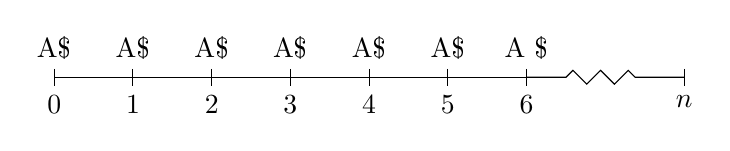
\begin{tikzpicture}[snake=zigzag, line before snake = 5mm, line after snake = 5mm]
    % draw horizontal line   
    \draw (0,0) -- (6,0);
    \draw[snake] (6,0) -- (8,0);

    % draw vertical lines
    \foreach \x in {0,1,2,3,4,5,6,8}
      \draw (\x cm,3pt) -- (\x cm,-3pt);

    % draw nodes
    \draw (0,0) node[below=3pt] {$ 0 $} node[above=3pt] {A\$};
    \draw (1,0) node[below=3pt] {$ 1 $} node[above=3pt] {A\$};
    \draw (2,0) node[below=3pt] {$ 2 $} node[above=3pt] {A\$};
    \draw (3,0) node[below=3pt] {$ 3 $} node[above=3pt] {A\$};
    \draw (4,0) node[below=3pt] {$ 4 $} node[above=3pt] {A\$};
    \draw (5,0) node[below=3pt] {$ 5 $} node[above=3pt] {A\$};
    \draw (6,0) node[below=3pt] {$ 6 $} node[above=3pt] {A \$};
    \draw (7,0) node[below=3pt] {$  $} node[above=3pt] {$ $};
    \draw (8,0) node[below=3pt] {$ n $} node[above=3pt] {$ $};
  \end{tikzpicture}
\begin{itemize}
\item La valeur future et présente d'une annuité de début de période pourra être trouvée en utilisant la formule pour l'annuité régulière avec un ajustement. 
\item En effet, la formule pour l'annuité régulière appliquée pour une annuité de début de période capitalisera l'ensemble des flux monétaire à $t=n-1$ pour la valeur future et actualisera l'ensemble des flux monétaire en $t=-1$ pour la valeur présente. 
\item Afin de déplacer $VF_{P_n}$ à $t=n$ et $VP_{P_0}$ à $t=0$, il faut multiplier la valeur présente et future de notre annuité régulière par $(1+r)$.
\end{itemize}
\end{frame}

\begin{frame}{Annuité de début de période}
\begin{block}{Valeur future d'une annuité de début de période $VF_{P_n^*}$}
\begin{align*}
VF_{P_n^*}=VF_{P_n} \times (1+r)
\end{align*}
\begin{align*}
VF_{P_n^*}=A \left[\frac{(1+r)^n-1}{r} \right] \times (1+r)
\end{align*}
\end{block}
\begin{block}{Valeur présente d'une annuité de début de période $VP_{P_0^*}$}
\begin{align*}
VP_{P_0^*}=VP_{P_0} \times (1+r)
\end{align*}
\begin{align*}
VP_{P_0^*}=A \left[ \frac{1-\frac{1}{(1+r)^n}}{r} \right] \times (1+r)
\end{align*}
\end{block}
\end{frame}

\begin{frame}{Déterminer le prix d'une obligation}
Dans cette section nous allons regarder comment trouver le prix de trois types d'obligations.
\begin{itemize}
\item Obligation régulière 
\item Obligation Zéro Coupon
\item Obligation perpétuelle
\end{itemize}
\end{frame}


\begin{frame}{Déterminer le prix d'une obligation}
\begin{block}{Obligation régulière}
Dans une obligation régulière un coupon est versé tous les semestres et le calcul du coupon est le suivant:
\begin{align*}
C= M * \frac{TC}{2}
\end{align*}
Où 
\begin{itemize}
\item $C=$ coupon semetriel 
\item $TC=$ taux de coupon annuel 
\item $M=$ Valeur nominal de l'obligation 
\end{itemize}

\end{block}
\end{frame}

\begin{frame}{Déterminer le prix d'une obligation}
\begin{block}{Obligation régulière}
Les flux monétaire d'une obligation peuvent être séparés en deux importantes composantes. 

\begin{enumerate}
\item Coupon payé de façon périodique jusqu'à l'échéance
\item Paiement de la valeur à l'échéance
\end{enumerate}
\vspace{1cm}
Le prix d'une obligation peut être également séparé en deux composantes:

\begin{enumerate}
\item la valeur actuelle des paiements de coupons semestriels
\item la valeur actuelle de la valeur à l'échéance 
\end{enumerate}
\end{block}
\end{frame}


\begin{frame}{Déterminer le prix d'une obligation}
\begin{block}{Obligation régulière}
Voici l'équation pour trouver le prix d'une obligation régulière:

\begin{align*}
P=\frac{C}{(1+r)^1}+\frac{C}{(1+r)^2}+...+\frac{C}{(1+r)^n}+\frac{M}{(1+r)^n}
\end{align*}

\begin{align*}
P=\sum_{t=1}^{n} \frac{C}{(1+r)^t}+\frac{M}{(1+r)^n}
\end{align*}

\end{block}
\end{frame}



\begin{frame}{Déterminer le prix d'une obligation}
\begin{block}{Obligation régulière}
On peut donc remarquer la présence d'une annuité dans la dernière équation 
\begin{align*}
\sum_{t=1}^{n} \frac{C}{(1+r)^t}=C \left[ \frac{1-\frac{1}{(1+r)^n}}{r} \right]
\end{align*}
On peut donc arriver à l'équation simplifiée pour le prix d'une obligation régulière.
\begin{align*}
P=C \left[ \frac{1-\frac{1}{(1+r)^n}}{r} \right]+\frac{M}{(1+r)^n}
\end{align*}

\end{block}
\end{frame}


\begin{frame}{Déterminer le prix d'une obligation}
\begin{block}{Obligation Zéro Coupon}
\begin{itemize}
\item Une obligation zéro coupon à la particularité de ne pas payer de coupons. 
\item Une obligation zéro coupon possède comme unique flux monétaire, la valeur actuelle de la valeur à l'échéance. 
\item On peut donc trouver le prix d'une obligation zéro coupon en actualisant seulement la valeur à l'écheance $M$. 
\end{itemize}
\begin{align*}
P_{zc}=\frac{M}{(1+r)^n}
\end{align*}
Où $P_{zc}$ représente le prix d'une obligation zéro coupon au temps $t=0$ venant à échéance après $n$ périodes 
\end{block}
\end{frame}


\begin{frame}{Déterminer le prix d'une obligation}
\begin{block}{Obligation perpétuelle}
\begin{itemize}
\item Une obligation perpétuelle à la particularité de ne pas avoir d'échéance. 
\item En effet, on suppose que les coupons seront payés pendant une période infinie. 
\item Sachant cela,  il nous possible de dire que la valeur d'une obligation perpétuelle est la suivante.
\end{itemize}
\begin{align*}
P_{p}=\sum_{t=1}^{\infty} \frac{C}{(1+r)^t}
\end{align*} 
Après manipulation de la dernière équation, il est possible d'arriver à l'expression suivante  pour le prix d'une obligation perpétuelle $P_p$.
\begin{align*}
P_p=\frac{C}{r}
\end{align*}
\end{block}
\end{frame}

\begin{frame}{Déterminer le prix d'une obligation}
\begin{block}{Prix d'une obligation entre deux dates de coupon}
\begin{itemize}
\item Il faut tout d'abord calculer le prix d'une obligation au moment où le dernier coupon a été versé. 
\item Si on suppose que le dernier coupon a été versé en t=0, alors le prix d'une obligation régulière à ce moment est trouvée comme suit:
\end{itemize}
\begin{align*}
P_0=C \left[ \frac{1-\frac{1}{(1+r)^n}}{r} \right]+\frac{M}{(1+r)^n}
\end{align*}
\end{block}
\end{frame}

\begin{frame}{Déterminer le prix d'une obligation}
\begin{block}{Prix d'une obligation entre deux dates de coupon}
\begin{itemize}
\item Le problème est que depuis le dernier coupon, une période de k s'est écoulée, alors le prix que nous venons de calculer est trop faible. 
\item Si le détenteur décidait de vendre sont obligation à $t= k$, au prix de $t=0$, il laisserait la totalité du prochain coupon au prochain acheteur.
\item Pour rectifier cette situation, il faut ajuster le prix $P_0$ pour tenir compte de l'intérêt accumulé entre $t=0$ et $t=k$. 
\item Il s'agit tout simplement de capitaliser le prix $P_0$ sur $k$ période. 
\end{itemize}
\begin{align*}
P_k=P_0 (1+r)^k
\end{align*}
\end{block}
\end{frame}

\begin{frame}{Déterminer le prix d'une obligation}
\begin{block}{Prix d'une obligation entre deux dates de coupon}
\begin{itemize}
\item Nous obtiendrons ainsi le prix reflétant l'intérêt accumulé $P_k$, appelé \textbf{full price} ou \textbf{dirty price}. 
\item On trouve ainsi l'équation complète afin de déterminer le prix d'une obligation entre deux paiements de coupons.
\end{itemize}
\begin{align*}
P_k= \left( C \left[ \frac{1-\frac{1}{(1+r)^n}}{r} \right]+\frac{M}{(1+r)^n} \right) \times (1+r)^k
\end{align*}
\end{block}
\end{frame}

\begin{frame}{Cotation}
Nous utiliserons le terme \textbf{cote} où \textbf{clean price} comme étant la valeur de l'obligation servant uniquement à rénumérer le vendeur de l'obligation pour la valeur intrinsèque. Pour trouver  ce prix, il faut soustraire les intérêts courrus au prix $P_k$.
\begin{align*}
cote_k=P_k-IC_k
\end{align*}
Où
\begin{itemize}
\item $cote_k=$ \textbf{clean price} à $t=k$
\item $P_k=$ \textbf{full price} ou \textbf{dirty price} à $t=k$
\item $IC_k=$ Intérêts courus à $t=k$
\end{itemize}

Pour trouver les intérêts courrus, il nous suffit de multiplier $k$ par la valeur du coupon périodique.
\begin{align*}
IC_k= k \times C
\end{align*}
\end{frame}

\begin{frame}{Convention pour la valeur de $k$}
Il est important de comprendre que $k$ possède comme unité de mesure, une période de coupon. Pour faciliter la compréhension, si on est exactement à mi-chemin entre deux versements de coupons, la valeur prise par $k$ sera de $0.5$. De façon très générale $k$ est déterminé avec la formule suivante:
\begin{align*}
k= \frac{N_{C_{t}}^{C_{t+k}}}{N_C}
\end{align*}
Où 
\begin{itemize}
\item $N_{C_{t}}^{C_{t+k}}$ est le nombre de jours depuis le dernier coupon. 
\item $N_C$ est le nombre de jours dans une période de coupon. 
\end{itemize}
\vspace{0.5cm}
De plus, tout dépendant du type d'obligation, une convention différente pour trouver la valeur de k sera appliquée.
\end{frame}

\begin{frame}{Convention pour la valeur de $k$}
\begin{block}{Titres gouvernementaux}
\begin{align*}
k=\frac{Exact}{Exact}
\end{align*}
\begin{itemize}
\item Numérateur : le nombre de jours exacts depuis le dernier coupon
\item Dénominateur : le nombre de jours exacts dans une période de coupon.
\end{itemize}
\end{block}
\end{frame}

\begin{frame}{Convention pour la valeur de $k$}
\begin{block}{Marché monétaire américain }
\begin{align*}
k=\frac{Exact}{360}
\end{align*}
\begin{itemize}
\item Numérateur : le nombre de jours exacts depuis le dernier coupon
\item Dénominateur : 360/nombre de coupons par année
\end{itemize}
\end{block}
\end{frame}

\begin{frame}{Convention pour la valeur de $k$}
\begin{block}{Obligations corporatives }
\begin{align*}
k=\frac{30}{360}
\end{align*}
\begin{itemize}
\item Numérateur : le nombre de jours depuis le dernier coupon en accordant aux mois entiers depuis le dernier coupon une valeur de 30 jours.
\item Dénominateur : 360/nombre de coupons par année
\end{itemize}
\end{block}
\end{frame}

\begin{frame}{Convention pour la valeur de $k$}
\begin{block}{Autre }
\begin{align*}
k=\frac{Exact}{365}
\end{align*}
\begin{itemize}
\item Numérateur : le nombre de jours exacts depuis le dernier coupon
\item Dénominateur : 365/nombre de coupons par année
\end{itemize}
\end{block}
\end{frame}

\begin{frame}{Relation Prix - Taux de rendement}
\begin{itemize}
\item Une obligation est émise avec un taux de coupon $TC$. 
\item Par la suite le rendement $y$, requis pour ce type d'obligation risque de varier dans le temps.
\item Le taux de rendement requis risque soit de surpasser le taux de coupon ou d'être inférieur à celui-ci. 
\end{itemize}
\end{frame}

\begin{frame}{Relation Prix - Taux de rendement}
Voici maintenant les trois possibilités pour la relation prix et taux de rendement. 
\begin{itemize}
\item Le taux de rendement requis surpasse le taux de coupon , ce qui rend le prix de notre obligation inférieur à la valeur nominale. 
\begin{itemize}
\item On dit que cette obligation est vendue à escompte 
\item $TC < y \rightarrow P < M$
\end{itemize}
\item Le taux de rendement requis devient inférieur au taux de coupon , ce qui rend le prix de notre obligation supérieur à la valeur nominale. 
\begin{itemize}
\item On dit que cette obligation est vendue à prime
\item $TC > y \rightarrow P > M$
\end{itemize}
\item Le taux de rendement requis reste égal au taux de coupon , ce qui rend le prix de notre obligation égale à la valeur nominale. 
\begin{itemize}
\item On dit que cette obligation est vendue au pair
\item $TC = y \rightarrow P = M$
\end{itemize}
\end{itemize}
\end{frame}

\begin{frame}{Relation Prix - Taux de rendement}
\begin{itemize}
\item On peut conclure en disant qu'il existe une relation inverse entre prix d'une obligation et son rendement. 
\item Il est important de comprendre que cette relation est également convexe.
\item En effet, une hausse du taux de rendement entraine une baisse de prix plus faible que la hausse de prix qu'entraine une baisse de taux équivalent.
\end{itemize}
\end{frame}

\end{document}
